\thispagestyle{quantoannone}
\pagestyle{quantoan}
\everymath{\color{quantoan}}
\graphicspath{{../quantoan/pic/}}
\blfootnote{\color{quantoan}\color{quantoan}$^*$Bài nói tại Viện hàn lâm Leopoldina của Berlin.}
\blfootnote{\color{quantoan}\color{quantoan}$^1$Freie Universität, Berlin.}
\begingroup
\AddToShipoutPicture*{\put(0,616){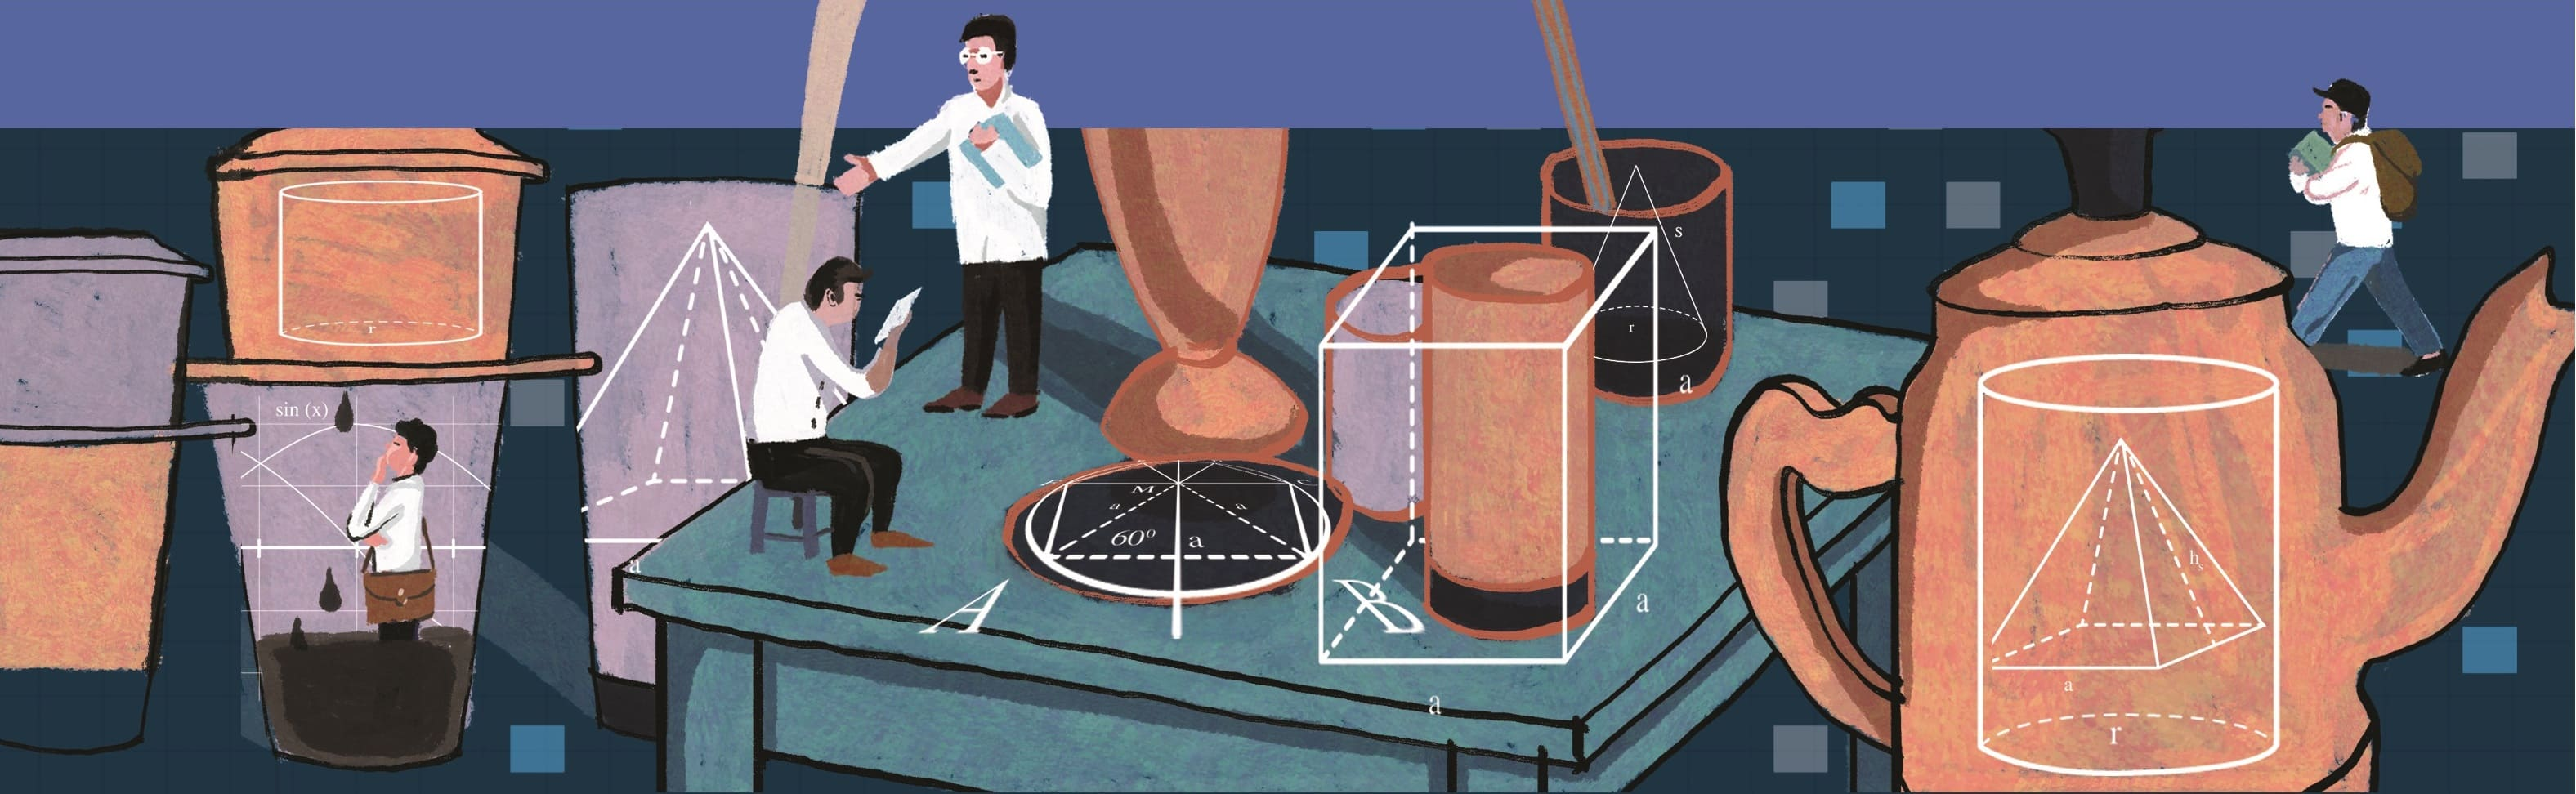
\includegraphics[width=19.3cm]{../bannerquantoan}}}
\AddToShipoutPicture*{\put(90,527){
\includegraphics[scale=1]{../tieude.pdf}}}
\centering
\endgroup

\vspace*{175pt}

\begin{multicols}{2}
	\textbf{\color{quantoan}Một lựa chọn nhỏ các trích dẫn}
	\vskip 0.1cm
	\textit{Wolfgang Goethe: Các nhà toán học là một kiểu người Pháp: nếu bạn nói chuyện với họ, họ sẽ dịch nó sang ngôn ngữ của họ, và sau đó nó sẽ sớm trở thành một thứ gì đó hoàn toàn khác. Goether thực sự không thích tiếng Pháp cũng như các nhà toán học (!) vì ông đã viết: Nền văn hóa mà toán học mang lại cho trí tuệ là vô cùng phiến diện và hạn chế.
	\begin{figure}[H]
		\vspace*{-5pt}
		\centering
		\captionsetup{labelformat= empty, justification=centering}
		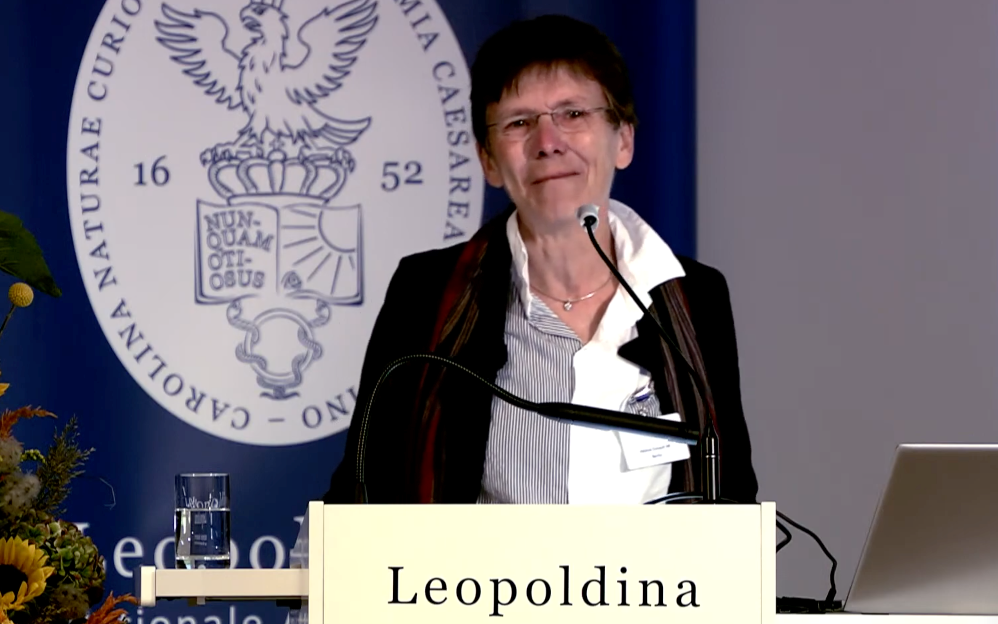
\includegraphics[width= 1\linewidth]{1aa}
		%		\caption{\small\textit{\color{}}}
		\vspace*{-15pt}
	\end{figure}
	Leonardo da Vinci: Bất cứ ai chỉ trích trí tuệ siêu phàm của toán học đều nuôi dưỡng sự nhầm lẫn.
	\vskip 0.1cm
	Cess Noteboom: Vì nghề nghiệp của mình, tôi đã quen với một số kiểu hoàn hảo nhất định. Một trong số đó là toán học. Toán học, nếu bạn tìm hiểu sâu hơn, có hình mái vòm của thơ ca, trong đó không có những điều không thể dự đoán trước, và nếu chúng ta thành thật mà nói, thì không có cả sự lầy lội của con người.  
	Albert Einstein: Toán học thuần túy, theo cách riêng của nó, là thi ca của những suy nghĩ logic.
	\vskip 0.1cm
	Karl Weierstrass: Đúng là một nhà toán học không có chút gì là thơ sẽ không bao giờ là một nhà toán học hoàn hảo.}
	\vskip 0.1cm
	\textbf{\color{quantoan}Tại sao chúng tôi làm toán?}
	\vskip 0.1cm
	Những con đường dẫn đến toán học có lẽ cũng nhiều như số người theo đuổi nó. Nhưng có một điều không đổi: toán học là tự do của chúng tôi. Một số người đến với toán học thông qua vật lý, một số người thông qua khoa học máy tính, một số người  thông qua kỹ thuật, một số người thông qua sinh học. Sẽ có lúc trong đời sống trí tuệ ta muốn sắp xếp lại những suy nghĩ của mình trước khi áp dụng chúng, hay khi ta muốn hiểu được nền tảng của chúng. Đó là sự hấp dẫn của sự trừu tượng, dù nó thường xa rời thực tế của thế giới bên ngoài.
	\vskip 0.1cm
	Những người khác đến với toán học thông qua nghệ thuật, thơ ca, triết học. Sẽ có thời điểm ta cố gắng vượt qua sự chủ quan trong thẩm mỹ. Đó là lúc ta cần tiêu chí ``đúng hoặc sai" của tựa đề bài viết. Chúng tôi phân biệt hai động cơ: ``trừu tượng" và ``đúng hoặc~sai".
	\vskip 0.1cm
	\textbf{\color{quantoan}Chúng tôi thực sự làm gì?}
	\vskip 0.1cm
	Chúng tôi thường bắt đầu khá trẻ. Với tôi, thời trẻ tôi đã bị lôi cuốn bởi sự trừu tượng, bao gồm cả điều ``đúng hoặc sai" này. Toán học buộc bạn phải suy nghĩ với những lập luận được xây dựng rõ ràng. Đó là một sự bảo vệ khỏi chủ nghĩa giáo điều. Toán học có thể cứu chúng ta khỏi sự thờ ơ với xã hội, xóa bỏ nỗi sợ hãi về tương lai và giải phóng chúng ta khỏi kỳ vọng mình sẽ có ích trong xã hội. Tất nhiên, toán học được xã hội hoan nghênh vì nó có ứng dụng, lấy ví dụ ChatGPT. 
	\vskip 0.1cm
	Nhiều người trong chúng ta cũng nỗ lực để lao động của họ có ứng dụng trong xã hội. Nhưng những người khác, trong đó có tôi, thì không. Tôi lớn lên dưới ảnh hưởng của Hiroshima và không bao giờ muốn làm bất cứ điều gì trong đời mà có thể gây ra hậu quả tàn khốc. Đó là lý do tại sao tôi quyết định nghiên cứu một thứ không mang lại kết quả gì cả: nghiên cứu trong ``lĩnh vực trừu tượng nhất" của toán học. Khi tôi nghĩ về toán học, thực tế của thế giới bên ngoài biến mất. Toán học hoạt động với các khái niệm khép kín. Một lý thuyết toán học dựa trên những ý tưởng phải tương thích với hàng nghìn ý tưởng đã được thêm vào cấu trúc toán học trước đó. Mỗi lý thuyết được ghi lại bằng một ngôn ngữ đặc biệt, thể hiện thông qua các định lý, mệnh đề, bổ đề, tất cả đều thuộc về các quy tắc chung của toán học và lý thuyết này được hỗ trợ bởi các chứng minh. 
	\vskip 0.1cm
	Điều bạn nhận được luôn là "đúng" hoặc "sai". Sai có thể là một lỗi logic, hoặc có thể được phát hiện từ sự không tương thích với một lý thuyết trước đó. Trong trường hợp sau, cũng có thể lý thuyết trước đó là sai. Đôi khi bạn tìm thấy lỗi trong những bài viết đã hơn 100 năm tuổi. Trong hầu hết các trường hợp, lỗi được phát hiện quá muộn là do lý thuyết cũ không còn quan trọng cho sự phát triển tiếp theo. Chúng tôi làm việc với những bài toán. Trong sự trừu tượng này, bản thân các bài toán đều xuất phát từ những suy nghĩ trừu tượng. Mỗi bước hiểu biết đều mang tới những bài toán mới, nó cứ tiếp diễn mãi. Các bài toán trong các lĩnh vực toán học thiên về ứng dụng hơn có thể đến từ toán học bên ngoài, nghĩa là, từ ``thực tế"...
	\vskip 0.1cm
	\textbf{\color{quantoan}Tại sao chúng tôi không cảm thấy mệt mỏi?}
	\vskip 0.1cm
	Một người bạn đã hỏi tôi như vậy gần đây. Tôi có hai ý để trả lời câu hỏi này. Một mặt, khi ta hiểu được một điều gì đó, dù nó rất nhỏ, thì niềm vui cũng vô cùng lớn lao, không gì có thể so sánh được. Không ai có thể tước đoạt điều đó từ ta. Thứ hai, chúng tôi muốn biết. Chúng tôi thực sự muốn biết. Tôi đã nói rằng, với tư cách là một nhà toán học tôi gặp khó khăn với một khái niệm trừu tượng của thực tế. Nhưng nếu bạn hỏi với tôi, hay nhiều người trong chúng tôi, thực tế chủ quan là gì, thì tôi sẽ trả lời: Mong muốn biết vô điều kiện. 
\end{multicols}
\vspace*{-10pt}
{\color{quantoan}\rule{1\linewidth}{0.1pt}}
\blfootnote{\color{quantoan}\color{quantoan}$^*$Theo The Economist.}
\blfootnote{\color{quantoan}\color{quantoan}$^1$Đại học Sư phạm Hà Nội.}
\begingroup
\AddToShipoutPicture*{\put(126,130){
\includegraphics[scale=1]{../tieude3.pdf}}}
\centering
\endgroup

\vspace*{25pt}

\begin{multicols}{2}
	Có một truyền thuyết  kể rằng thành phố Portland, bang Oregon đã suýt được gọi là Boston. Cuối cùng thì vấn đề đã được quyết định nhờ một cuộc tung đồng xu được tổ chức vào năm $1845$ giữa Francis Pettygrove, người đến từ một thành phố Portland khác, ở bang Maine, và Asa Lovejoy, đến từ Boston (ở bang Massachusetts). Nhưng mọi chuyện có thể đã khác đi, theo Frantisek Bartos, một sinh viên tốt nghiệp tại Đại học Amsterdam, nếu con người chúng ta  không phải là những người tung xu một cách lưỡng lự thiếu dứt khoát như vậy.
	\begin{figure}[H]
		\vspace*{-5pt}
		\centering
		\captionsetup{labelformat= empty, justification=centering}
		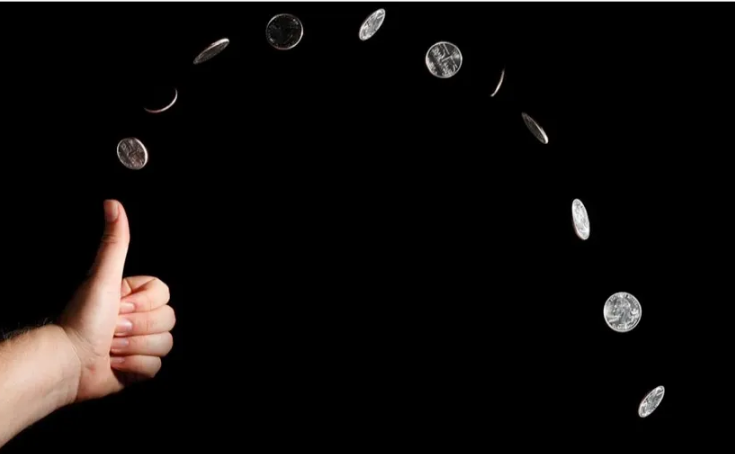
\includegraphics[width= 1\linewidth]{1111}
		%		\caption{\small\textit{\color{}}}
		\vspace*{-15pt}
	\end{figure}
	Bartos đã quan tâm đến một dự đoán hấp dẫn của Persi Diaconis, Susan Holmes và Richard Montgomery, một nhóm các nhà toán học người Mỹ. Trong một bài báo đăng vào năm $2007$, bộ ba này đã phân tích tính chất vật lý của việc tung đồng xu và nhận thấy có một điều gì đó khá hấp dẫn. Bên cạnh việc khiến đồng xu quay lộn nhào, hầu hết mọi người đều có xu hướng tạo ra một sự xoay nhẹ cho đồng xu khi họ tung nó. Điều đó làm cho trục xuay mà đồng xu lật quanh đó sẽ bị trôi đẩy khi nó ở trên không trung, một hiện tượng gọi là tuế sai.
	\vskip 0.1cm
	Kết quả cuối cùng, khi các con số được xử lý, là: một đồng xu do con người ném sẽ thể hiện một xu hướng thiên lệch khá tinh tế nhưng bền vững. Tiến sĩ Diaconis và các đồng nghiệp của ông tính toán có khoảng $51\%$ khả năng một đồng xu sẽ rơi theo hướng như trước khi được ném. Nói cách khác, nếu nó ngửa trong tay người ném, có nhiều khả năng hơn một chút là nó cũng sẽ chạm đất ngửa. Hoặc ít nhất, đó cũng là dự đoán.
	\vskip 0.1cm
	Bartos cùng với sự nhiệt tình đáng ngưỡng mộ của mình bắt tay vào kiểm tra thực nghiệm. Anh đã tập hợp được $48$ tình nguyện viên và thuyết phục họ thực hiện (và có quay phim) $350{.}707$ lần tung đồng xu, sử dụng hàng chục đồng xu khác nhau, từ đồng hai rupee của Ấn Độ đến đồng xu hai franc Thụy Sỹ. Dĩ nhiên, dữ liệu của anh  đã xác nhận những gì vật lý đã dự đoán. Các đồng xu đã chạm đất cùng với mặt khi tung lên tới tận $50,8\%$ số lần được ném.
	\vskip 0.1cm
	Số liệu thống kê chỉ ra rằng bản thân các đồng xu không có sự thiên lệch cụ thể nào. Yếu tố quyết định thực sự là con người chúng ta rõ ràng không có khả năng ném thẳng.  Bartos không phải là người đầu tiên thu thập số liệu thống kê về việc tung đồng xu. Nhưng anh ta là người đầu tiên làm được điều đó ở quy mô đủ lớn để phát hiện ra sự thiên lệch. (Một nỗ lực trước đó gồm $40{.}000$ lần tung, do hai sinh viên tại Đại học California tại Berkeley  thực hiện, đã thiếu sức mạnh thống kê để xác nhận được  lý thuyết.)
	\vskip 0.1cm
	Cơ hội $50,8\%$ chỉ khác một chút so với mức công bằng hoàn hảo. Nhưng  Bartos chỉ ra rằng cơ hội đó lớn hơn cả  lợi thế mà một sòng bạc có được trong hầu hết các loại kiểu chơi blackjack. Và trong một số tình huống cơ hội đó có thể có vai trò quan trọng. Vào năm $2019$, Sue Cudilla trở thành thị trưởng của Araceli, một thị trấn ở Philippines, nhờ việc tung đồng xu sau khi cuộc bầu cử được tuyên bố là bất phân thắng bại. Quan trọng hơn nữa, việc tung đồng xu có thể xác định ai là người ném bóng hoặc đánh bóng trước trong môn cricket. Các vận động viên chuyên nghiệp luôn chi hàng nghìn đô--la  và hàng giờ tập luyện để tìm kiếm được những lợi thế cận biên. Có lẽ họ giờ  sẽ phải nên chú ý nhìn vào đồng xu lẻ trong túi quần của trọng tài.
\end{multicols}